\begin{figure} [h!]
\begin{center}

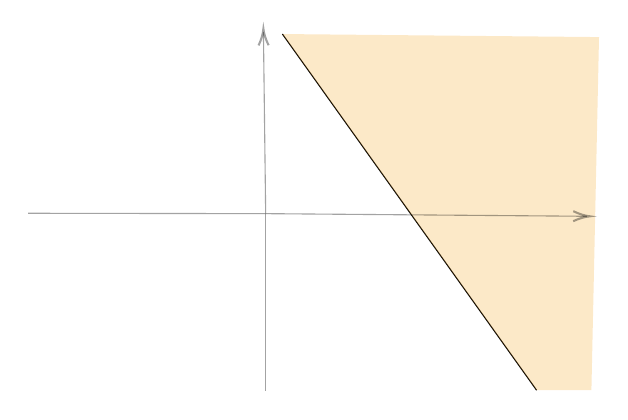
\begin{tikzpicture}[x=0.55pt,y=0.55pt,yscale=-1,xscale=1]
%uncomment if require: \path (0,300); %set diagram left start at 0, and has height of 300

%Straight Lines [id:da834373648885985] 
\draw    (335,25.5) -- (502,259.5) ;
%Shape: Polygon [id:ds19097348090692345] 
\draw  [draw opacity=0][fill={rgb, 255:red, 245; green, 166; blue, 35 }  ,fill opacity=0.25 ] (543,27.5) -- (538,259.5) -- (502,259.5) -- (335,25.5) -- cycle ;
%Straight Lines [id:da488242538610719] 
\draw [color={rgb, 255:red, 0; green, 0; blue, 0 }  ,draw opacity=0.36 ]   (324,143.5) -- (322.52,24) ;
\draw [shift={(322.5,22)}, rotate = 449.29] [color={rgb, 255:red, 0; green, 0; blue, 0 }  ,draw opacity=0.36 ][line width=0.75]    (10.93,-3.29) .. controls (6.95,-1.4) and (3.31,-0.3) .. (0,0) .. controls (3.31,0.3) and (6.95,1.4) .. (10.93,3.29)   ;
%Straight Lines [id:da1979668435494064] 
\draw [color={rgb, 255:red, 0; green, 0; blue, 0 }  ,draw opacity=0.36 ]   (324,143.5) -- (324,260.25) ;
%Straight Lines [id:da5494641877725677] 
\draw [color={rgb, 255:red, 0; green, 0; blue, 0 }  ,draw opacity=0.36 ]   (168,143.25) -- (324,143.5) ;
%Straight Lines [id:da7425835818655306] 
\draw [color={rgb, 255:red, 0; green, 0; blue, 0 }  ,draw opacity=0.36 ]   (324,143.5) -- (535,145.23) ;
\draw [shift={(537,145.25)}, rotate = 180.47] [color={rgb, 255:red, 0; green, 0; blue, 0 }  ,draw opacity=0.36 ][line width=0.75]    (10.93,-3.29) .. controls (6.95,-1.4) and (3.31,-0.3) .. (0,0) .. controls (3.31,0.3) and (6.95,1.4) .. (10.93,3.29)   ;

\end{tikzpicture}

\end{center} 
% \caption{Visualization of trajectory generation done in the developed software}
\end{figure}